\documentclass[spanish,11pt,a4paper]{article}

\usepackage[utf8]{inputenc}
\usepackage{amsmath}
\usepackage[a4paper]{geometry}
\usepackage{graphicx}
\usepackage{subfigure}
\usepackage{tikz}
\usetikzlibrary{shapes,arrows}

\title{\Huge Práctica 2}
\date{\today}
\author{Víctor Galvín Coronil}

\tikzstyle{block} = [draw, fill=white, rectangle, 
    minimum height=3em, minimum width=6em]
\tikzstyle{sum} = [draw, fill=white, circle, node distance=1cm]
\tikzstyle{input} = [coordinate]
\tikzstyle{output} = [coordinate]
\tikzstyle{pinstyle} = [pin edge={to-,thin,black}]

\begin{document}

\section{Diagrama de Bloques} 

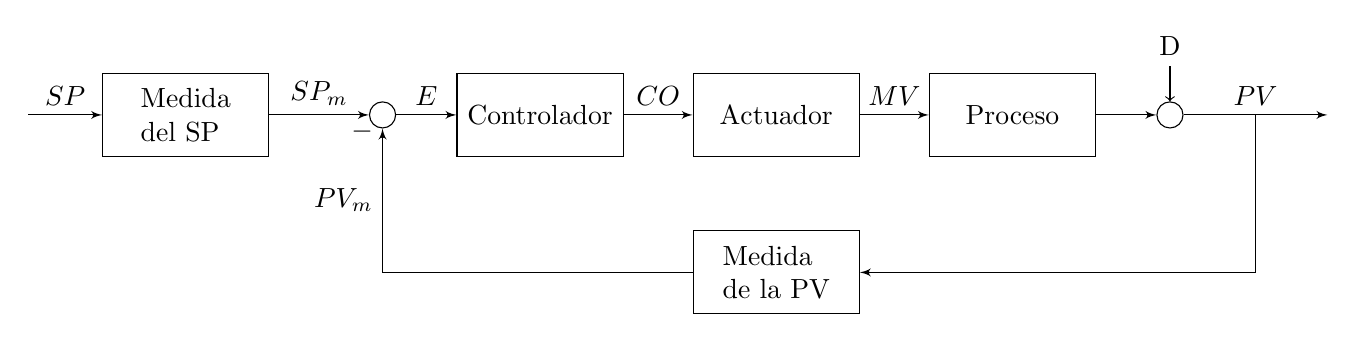
\begin{tikzpicture}[auto, node distance=2cm,>=latex']

    \node [input, name=input] {};
    \node [block, right of=input, align=left] (medida_st) {Medida \\ del SP};
    \node [sum, right of=medida_st, node distance=2.5cm] (sum) {};
    \node [block, right of=sum] (controlador) {Controlador};
    \node [block, right of=controlador, node distance=3cm] (actuador) {Actuador};
    \node [block, right of=actuador, 
            node distance=3cm] (proceso) {Proceso};
    \node [sum, right of=proceso, pin={[pinstyle]above:D}, node distance=2cm] (sum2) {};

    \draw [->] (controlador) -- node[name=u] {$CO$} (actuador);
    \draw [->] (actuador) -- node[name=u] {$MV$} (proceso);
    \draw [->] (proceso) -- node[name=u] {} (sum2);
    \node [output, right of=sum2] (output) {};
    \node [block, below of=actuador, align=left] (medida) {Medida \\ de la PV};

    \draw [draw,->] (input) -- node {$SP$} (medida_st);
    \draw [->] (medida_st) -- node {$SP_m$} (sum);
    \draw [->] (sum) -- node {$E$} (controlador);
    \draw [->] (sum2) -- node [name=y] {$PV$}(output);
    \draw [->] (y) |- (medida);
    \draw [->] (medida) -| node[pos=0.99] {$-$} 
        node [near end] {$PV_m$} (sum);
\end{tikzpicture}

\end{document}